\documentclass[10pt]{beamer}
\usetheme{Boadilla} % My favorite!
\setbeamercovered{invisible}
% To remove the navigation symbols from 
% the bottom of slides%
\setbeamertemplate{navigation symbols}{} 
\setbeamertemplate{itemize items}[default]
\setbeamertemplate{enumerate items}[default]
\xdefinecolor{lavendar}{rgb}{0.2, 0.2, 0.72}
%
\usepackage{graphicx,epsfig}

%\usepackage{bm}         % For typesetting bold math (not \mathbold)
%\logo{\includegraphics[height=0.6cm]{yourlogo.eps}}
%
\newcommand{\be}{\begin{equation*}}
\newcommand{\ee}{\end{equation*}}
\newcommand{\ba}{\begin{eqnarray}}
\newcommand{\ea}{\end{eqnarray}}

\newcommand{\vso}{\vskip15pt}
\newcommand{\vst}{\vskip30pt}
\newcommand{\nsub}{n_\mathrm{sub}}

\usepackage{listings}
\usepackage{color}
\usepackage{textcomp}
\definecolor{listinggray}{gray}{0.9}
\definecolor{lbcolor}{rgb}{1,1,1}
\lstset{
	backgroundcolor=\color{lbcolor},
	tabsize=4,
	rulecolor=,
	language=matlab,
        basicstyle=\scriptsize,
        upquote=true,
        aboveskip={1.5\baselineskip},
        columns=fixed,
        showstringspaces=false,
        extendedchars=true,
        breaklines=true,
        prebreak = \raisebox{0ex}[0ex][0ex]{\ensuremath{\hookleftarrow}},
        frame=single,
        showtabs=false,
        showspaces=false,
        showstringspaces=false,
        identifierstyle=\ttfamily,
        keywordstyle=\color[rgb]{0,0,1},
        commentstyle=\color[rgb]{0.133,0.545,0.133},
        stringstyle=\color[rgb]{0.627,0.126,0.941},
}

\def\smallfrac#1#2{\hbox{${{#1}\over {#2}}$}}

\title[]{Interpolation tools for NLO calculation with event generators}
\author{Nathan Hartland}
\institute
{
Universit\"at G\"ottingen\\
%
\includegraphics[height=2cm]{edinburghcrest.pdf}
\medskip
}
% \today will show current date. 
% Alternatively, you can specify a date.
%

\date{\today}


\begin{document}
\renewcommand{\inserttotalframenumber}{13}


\begin{frame}
\begin{centering}
\vskip20pt
\center{\huge\color{lavendar} \textbf{Interpolation tools for NLO calculation with event generators}}
\vskip30pt
Nathan Hartland\\
\small{Georg-August Universit\"at G\"ottingen}\footnote{
Funding provided by MCnet Short-term studentship.}\\
\small{and The University of Edinburgh}\\
\vskip50pt
MCNet network meeting\\
Manchester, UK,\\
October 29th, 2013.
\vskip15pt

\includegraphics[height=1.0cm]{glogo.eps} \hfill

\includegraphics[height=1.0cm]{edinburghcrest.pdf}


\end{centering}

\end{frame}

\section{Parton distribution fitting}
\begin{frame}
\frametitle{PDF/$\alpha_S$/Scale variations with MC events}
Changing the QCD variables present in a MC calculation is a problem with a classic space-time tradeoff.
\vso
One can either: \vskip5pt
\begin{itemize}
		\item<1-> Rerun the event generation with the relevant quantities modified (time)
		\item<1-> Store the full event record of the calculation and reweight the events (space)
\end{itemize}
\vskip5pt
As rerunning the MC becomes impractical in high statistics/expensive runs, event reweighting is usually the way to go.
\vskip5pt

\be \sigma = \sum_i^{N_{evt}} w_i\left(Q^2_i,\alpha_S\left(  Q^2_i\right) \right)f^{(1)}_i\left(x^1_i, Q^2_i\right)f^{(2)}_i\left(x^1_i, Q^2_i\right) .  \ee
\vskip5pt

However, lots of storage required, actual PDF dependence may be rather more complicated, still rather slow (for applications such as PDF fitting).

\end{frame}

\begin{frame}
\frametitle{Interpolation tools for MC calculations}
\underline{Possible solution}: \\
Store your MC weights upon an interpolating grid in PDF $x$ and $Q^2$ \\
\begin{itemize}
\item<1-> Equivalent to using an interpolated form of your PDFs.
\end{itemize}

\begin{equation} \nonumber
\label{eq:applconv}
\sigma = \sum_p \sum_{i,j}^{N_{\mathrm{pdf}}} \sum_{\alpha,\beta}^{N_x} \sum_{\tau}^{N_{Q}}
W_{ij\alpha\beta\tau}^{(p)} \, \left( \frac{\alpha_s\left(Q^2_{\tau}\right)}{2\pi}\right)^{p}
f_{i}\left(x_{\alpha},  Q^2_{\tau}\right)f_{j}\left(x_{\beta},  Q^2_{\tau}\right)
\end{equation}
\vskip5pt
Varying your parameters is a simpler exercise after determining the weight grid $W$.
\vso
A number of solutions have been on the market for a while now. \\
\begin{itemize}
\item<1-> Good examples are the FastNLO and APPLgrid projects.
\end{itemize}
\vskip5pt
The APPLgrid package provides:
\begin{itemize}
\item<1->  a general structure for doing these products and variations.
\item<1->  an interface to populate a weight grid $W$ with MC events.
\end{itemize}
\end{frame}


\begin{frame}
\frametitle{Project outline}
At the present, working interfaces to the APPLgrid software are only available from the NLO codes MCFM and nlojet++.
\vso

\underline{Proposal:} 
\vskip4pt
Construct an interface for SHERPA to APPLgrid in order to:
\begin{itemize}
\item<1-> Aid in performing systematic studies of NLO calculations with SHERPA.
\item<1-> Permit access to cutting edge one-loop tools in performance sensitive applications such as PDF fitting.
 \end{itemize}
 
 \vskip15pt
\underline{Implementation:}\\
\vskip4pt
Three points must be addressed in such an interface.
\begin{itemize}
\item<1-> Classification of the event's initial state.
\item<1-> Classification of the event's final state.
\item<1-> Conversion of the provided weight into an APPLgrid fill call.

\end{itemize}

\end{frame}


\begin{frame}
\frametitle{Implementation - subprocess classification}

\begin{itemize}
\item<1-> Classification of the event's initial state.
\end{itemize}

Sherpa generates events fully exclusive in the initial state
(i.e individual parton-parton combinations rather than QCD subprocesses).

\be F^{(l)}\left(x_1,x_2,Q^2\right) = \sum_{ij}^{N_{fl}} C^{(l)}_{ij} \, f_i\left(x_1,Q^2\right) f_j\left(x_2,Q^2\right). \ee

APPLgrid allows for the grouping of initial state combinations that only differ by their PDFs. 

\begin{itemize}
\item<1-> Reduces file size (121 $\to$ $N_{sub}$ grids).
\item<1-> Reduces final convolution time.
\end{itemize}
\vskip10pt

\underline{Implementation:}\\
\vskip4pt
SHERPA provides the required mapping information, which can be converted into
a APPLgrid subprocess configuration file with a provided script. Scripts are provided for both COMIX and AMEGIC.
%{ \small
%\underline{Important note:}\\
%Subprocess grouping requires a rather careful treatment of the generated event statistics.
%Results shown here are without subprocess grouping, as only then can we make direct comparison
%to the benchmark (rivet) result.}

\end{frame}

\begin{frame}
\frametitle{Implementation - final state classification}

\begin{itemize}
\item<1-> Classification of the event's final state.
\end{itemize}
\vskip10pt
A new interface requires a suite of analysis tools to convert event final states and weights into
appropriately binned observables for comparison with experimental data.
 \vso
 \underline{Implementation:}\\
\vskip4pt
Design the interface as a plugin for the Rivet MC analysis system:
\vskip5pt
\begin{itemize}
\item<1-> Interface based upon HepMC records $\to$ (relatively) generator indepenendant.
\item<1-> Experimental binning and data comparison provided by standard Rivet formats.
\item<1-> Analysis implementation as standard in Rivet, simply fill APPLgrid in parallel with histograms.
\end{itemize}

\end{frame}

\begin{frame}
\frametitle{Implementation}
\begin{itemize}
\item<1-> Conversion of the provided weight into an APPLgrid fill call.
\end{itemize}
\vskip5pt
Rivet analyses are based upon HepMC records\\
\quad\quad$\to$ by design mostly final state information.
\vskip15pt
On top of the standard HepMC information, also required:
\begin{itemize}
\item<1-> Power of $\alpha_S$ characterising the event.
\item<1-> Full breakdown of the weight's PDF dependance.
\end{itemize}
\vskip15pt
In Sherpa v2.0 the HepMC short record type now includes this information in the user weights container.
\vskip15pt
PDF dependence is detailed using the same basis as used in the Sherpa NTuple format.

\end{frame}

\begin{frame}[fragile]
\frametitle{Analysis example}
\begin{itemize}
\item<1-> Write your Rivet analysis as usual.
\item<1-> In the initialisation phase, book your subprocess PDF and grid objects:
\end{itemize}
\vskip-10pt
\begin{lstlisting}[language=c++]
     // book the APPLgrid PDF combination
     bookPDF("subprocess.config");

     histo = bookHisto1D(1, 1, 1);
     grid  = bookGrid(histo, histoDir(), "subprocess.config", 
                      LOpower, xmin, xmax, Q2min, Q2max);

\end{lstlisting}
\begin{itemize}
\item<1-> In the analysis phase, fill your grid in parallel with your histogram.
\end{itemize}
\vskip-10pt

\begin{lstlisting}[language=c++]
     histo->fill(coordinate, weight);        
     grid->fill(coordinate, event);
\end{lstlisting}

\begin{itemize}
\item<1-> In the finalise phase, normalise and export your grid.
\end{itemize}
\vskip-10pt
\begin{lstlisting}[language=c++]
     scale(histo, crossSection()/sumOfWeights());
     grid->scale(crossSection()/sumOfWeights());
      
     grid->exportgrid();
\end{lstlisting}

\end{frame}

\begin{frame}
\frametitle{Validation - DY }
Generate 100M ppbar DY Events.\\
\begin{itemize}
\item<1-> Process events with Rivet CDF Z Rapidity analysis into an APPLgrid.
\item<1-> Reconvolute with original PDF (CT10) and compare against benchmark cross section.
\end{itemize}
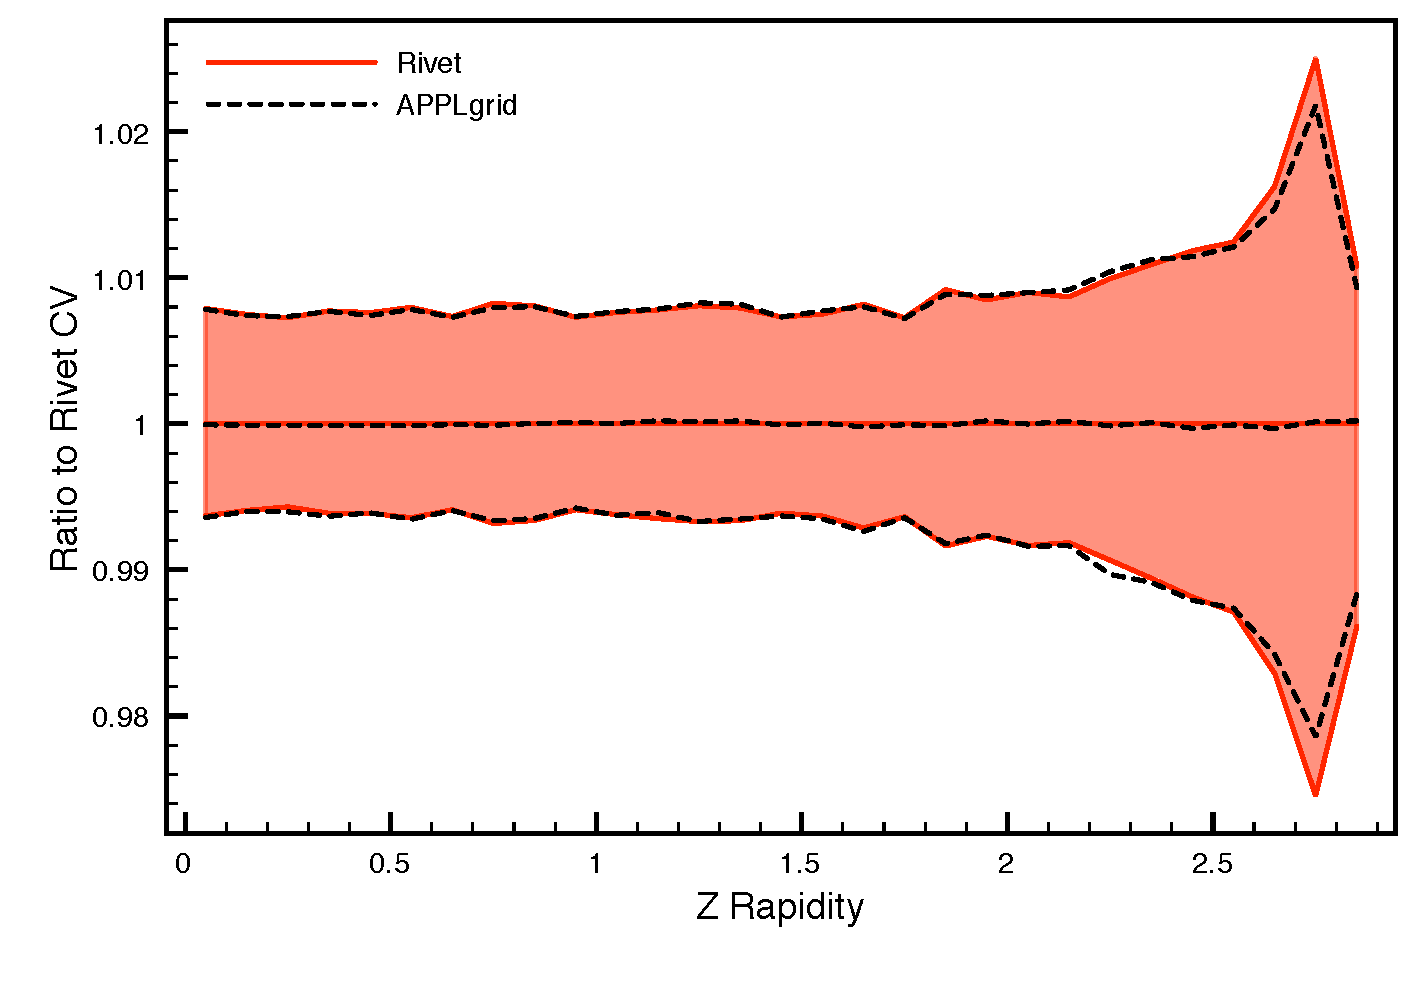
\includegraphics[width=0.45\paperwidth]{100MDYScales_Plot.pdf}
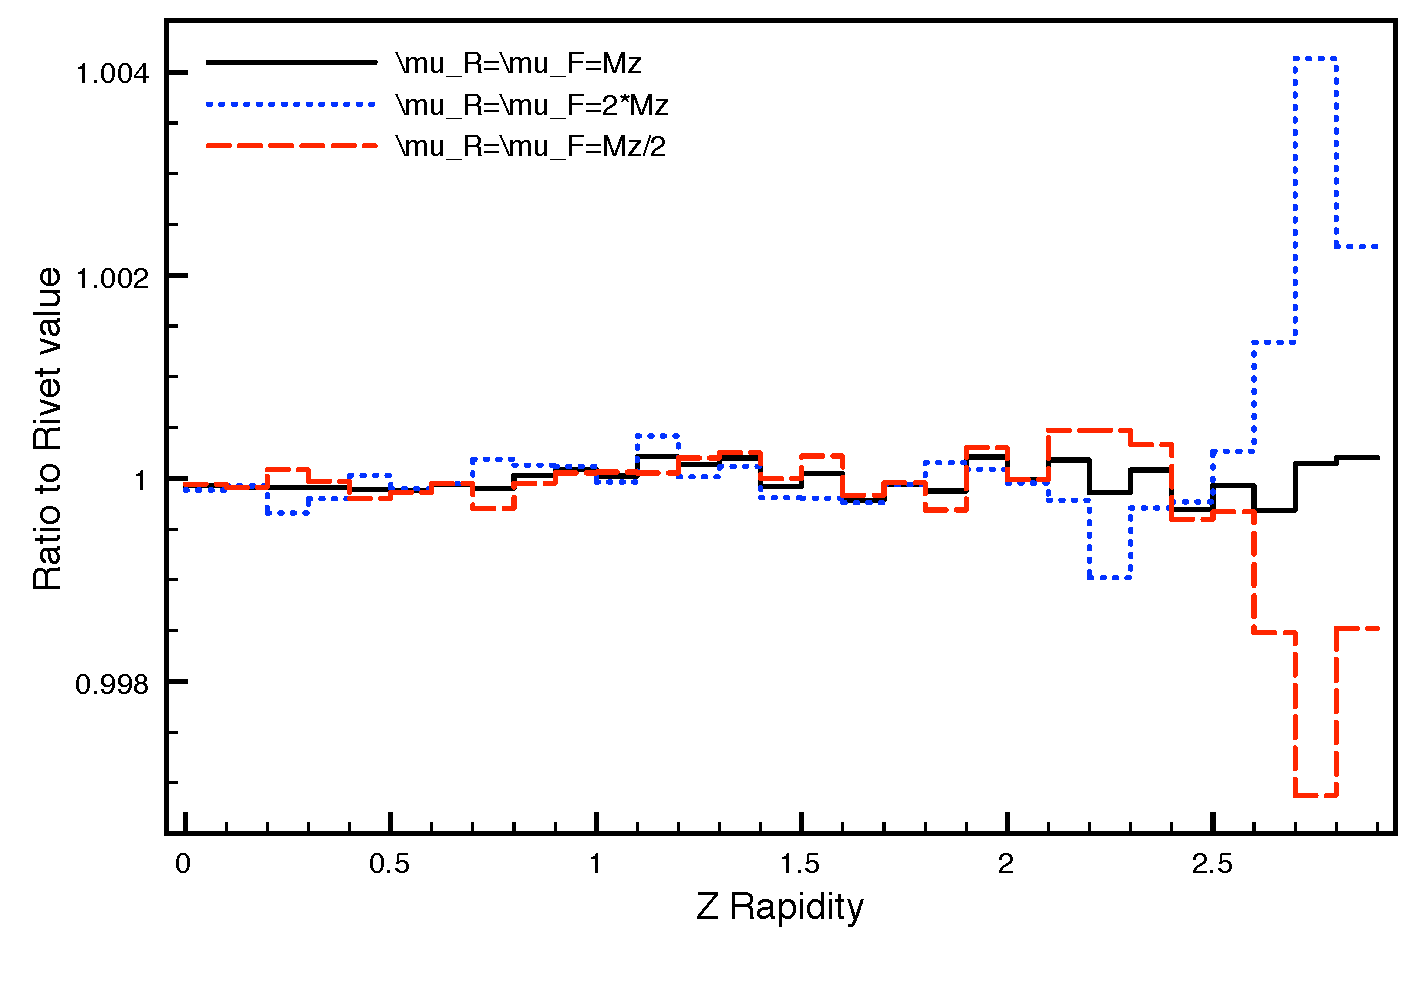
\includegraphics[width=0.45\paperwidth]{100MDYRatioScales_Plot.pdf}

\begin{itemize}
\item<1-> Excellent reproduction of rivet result.
\item<1-> APPLgrid result for scale variation also in agreement with separate Sherpa runs.
\end{itemize}
\end{frame}

\begin{frame}
\frametitle{Validation - DY PDF variation}
Use APPLgrid generated with CT10 PDF to make predictions with MSTW08.
\vso

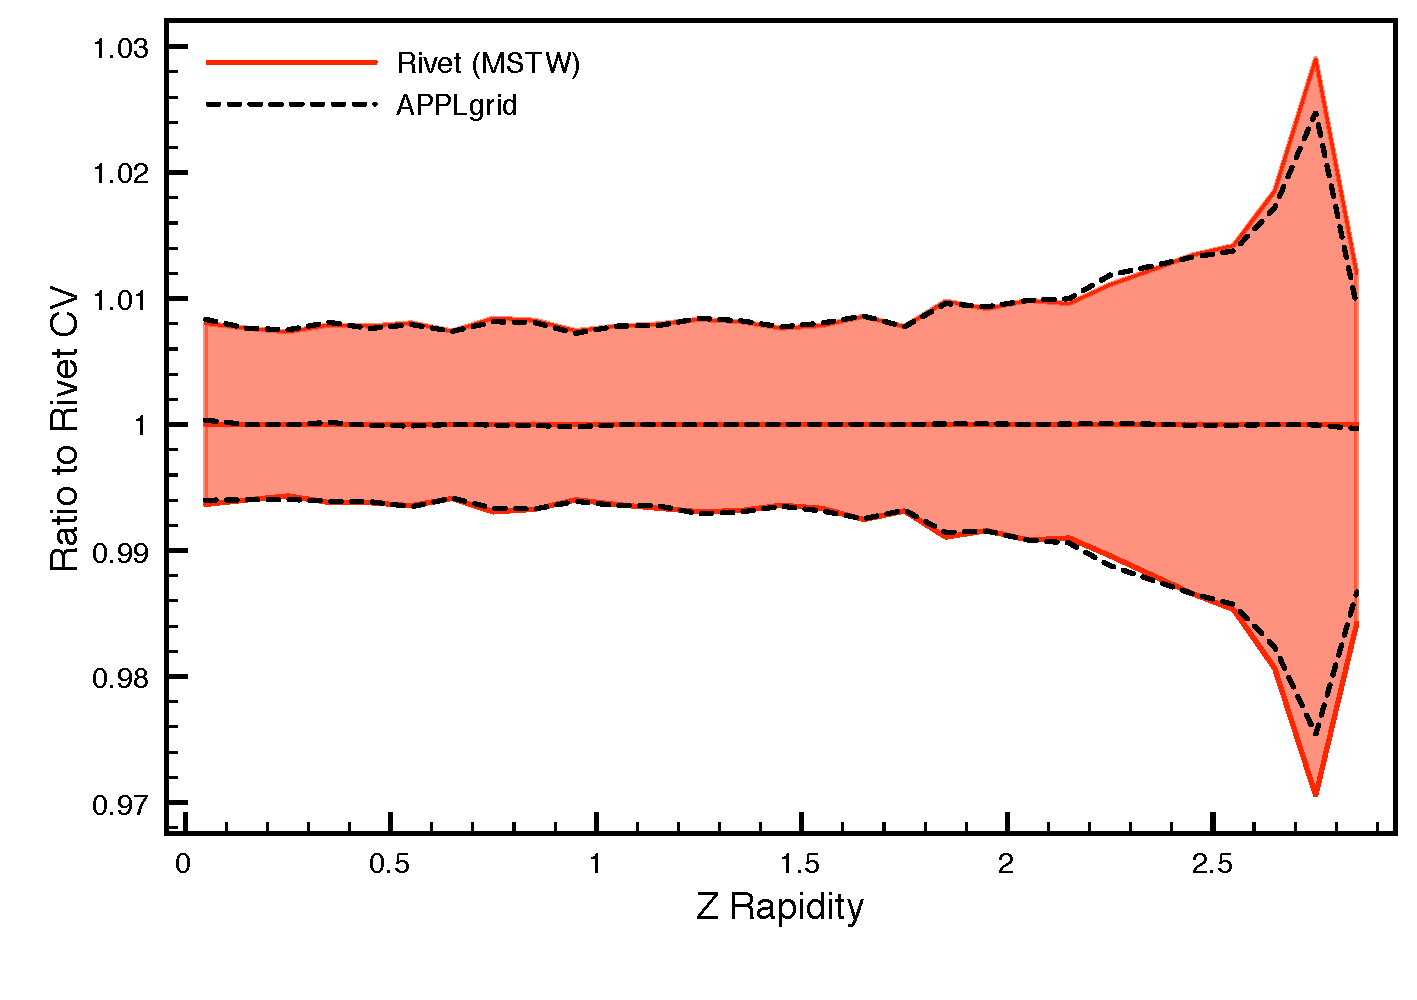
\includegraphics[width=0.45\paperwidth]{100MDYMSTW_Plot.pdf}
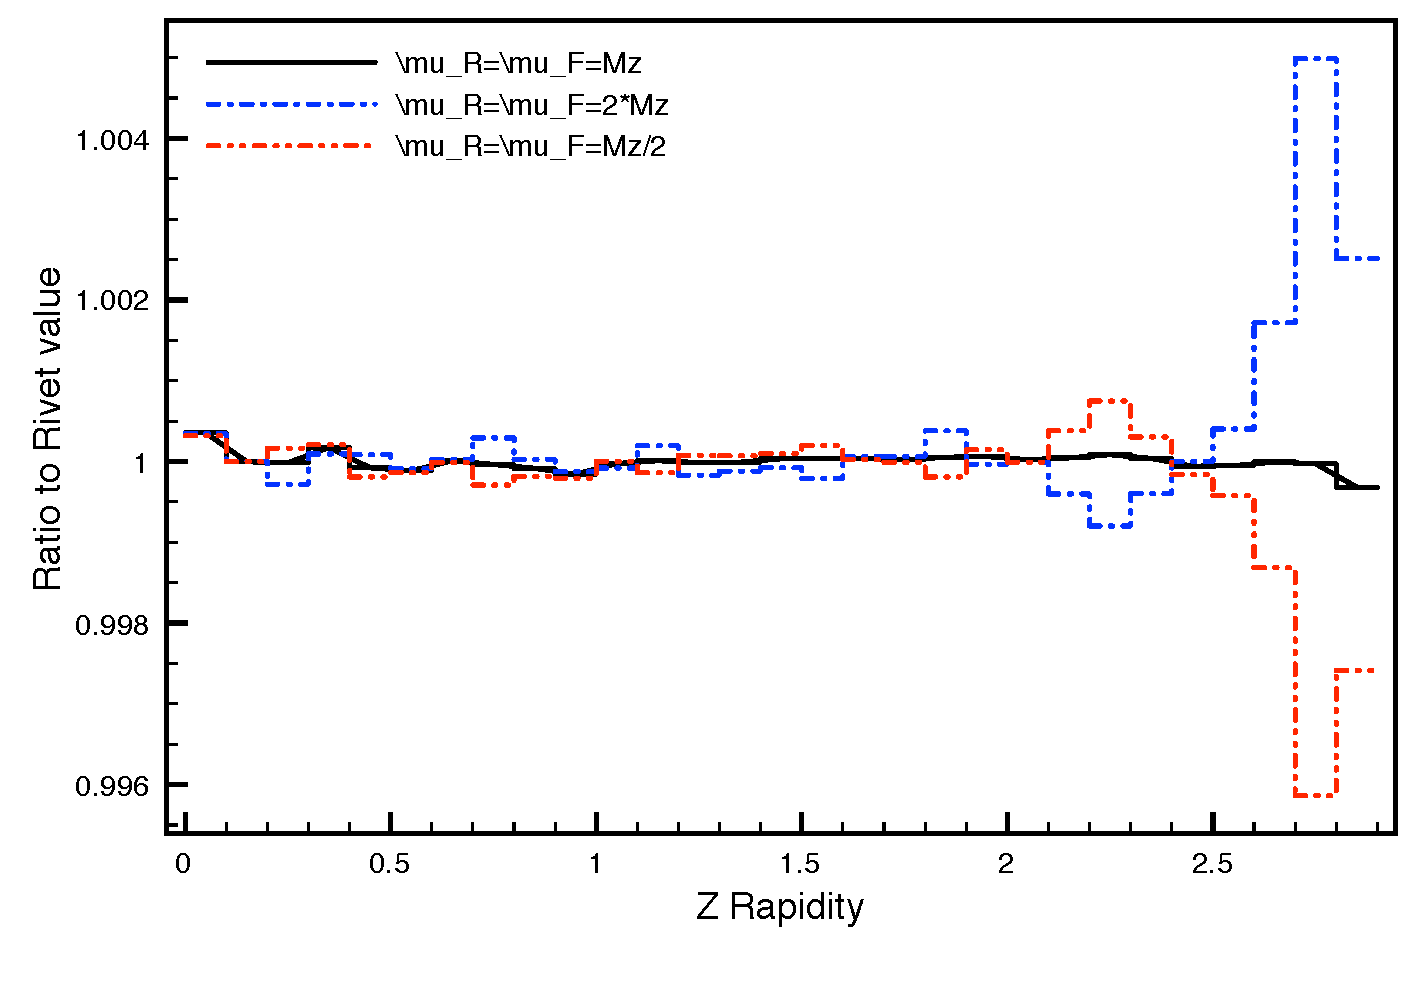
\includegraphics[width=0.45\paperwidth]{100MDYRatioMSTW_Plot.pdf}
\vso
\begin{itemize}
\item<1-> APPLgrid is able to efficiently reweight with MSTW08 PDFs.
\item<1-> Good reproduction of both central values and scale variations.
\end{itemize}
\end{frame}

\begin{frame}
\frametitle{Validation - Inclusive Jets}
Generate 100M pp Dijet events. 
\begin{itemize}
\item<1-> Vary interpolation grid to assess control over errors.\\
\end{itemize}

\centering{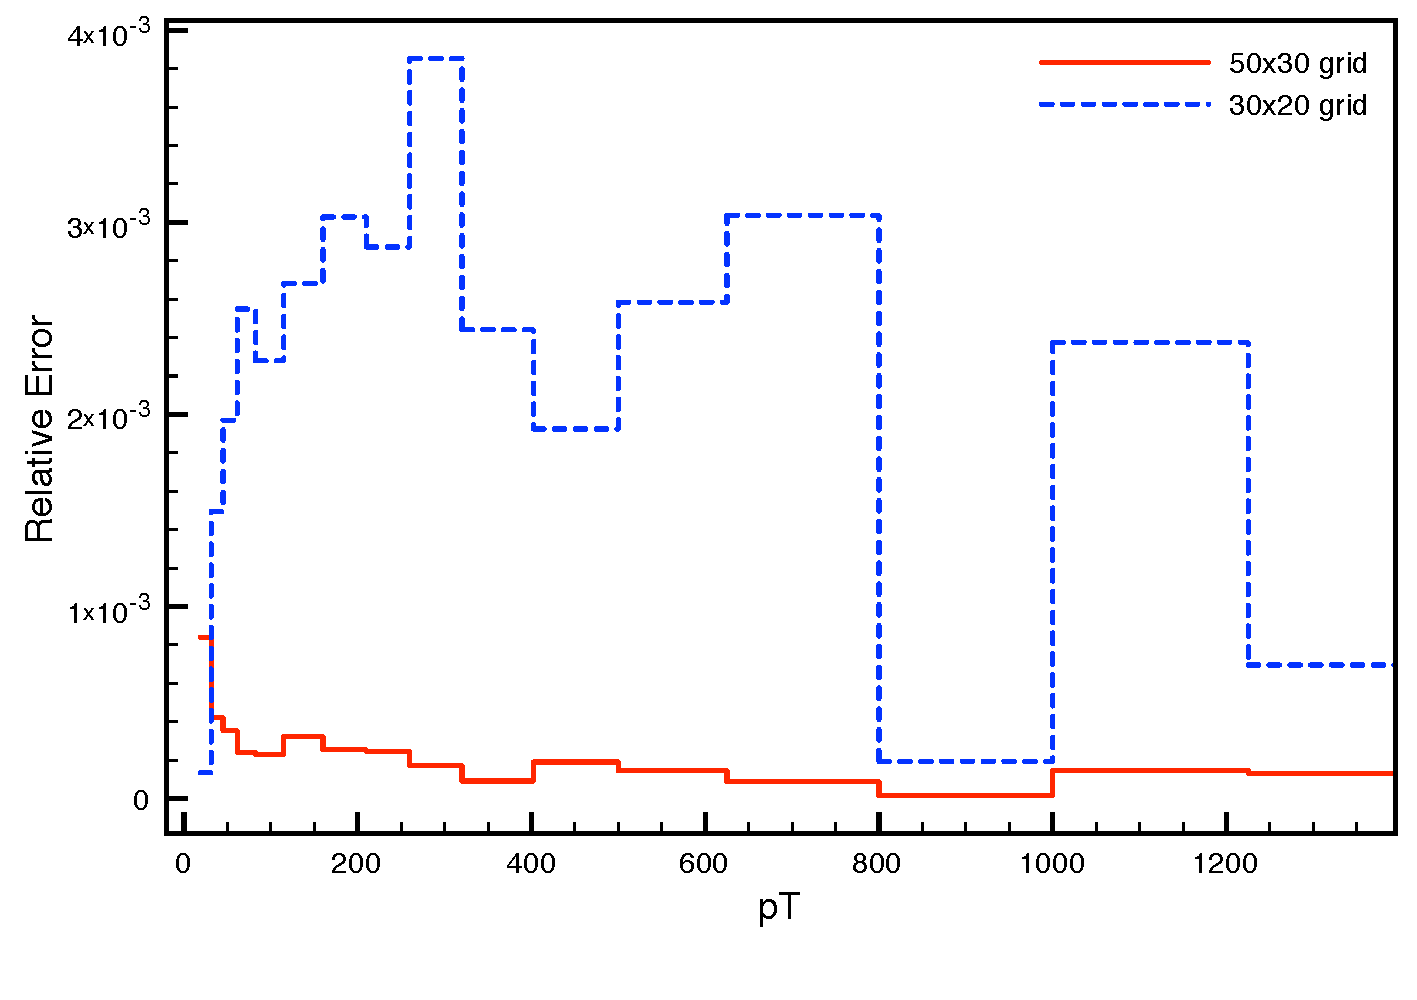
\includegraphics[width=0.6\paperwidth]{GridDep_Jets.pdf}}

\begin{itemize}
\item<1-> APPLgrid is able to reproduce the central value prediction to better than permil accuracy.
\item<1-> Discrepancies may be controlled to user's requirements by using finer grids.
\end{itemize}

\end{frame}


\begin{frame}
\frametitle{Conclusion}
We have developed an interface for event generators (Sherpa) to the APPLgrid NLO interpolation framework.\\
\vskip10pt
This interface allows for the efficient variation of parameters in an NLO QCD calculation, such as
\begin{itemize}
\item<1-> $\alpha_S$.
\item<1-> Parton distributions.
\item<1-> Renormalisation and factorisation scales.
\end{itemize}
\vskip10pt
Without the need to store large event records.
\vskip10pt
Interface will be provided as a package in which the user may design modified rivet analyses, to be
installed as standard rivet plugins.

\vskip15pt
\center{ \textbf{Many thanks to MCNet for providing the funding for this project.} }

\end{frame}


\begin{frame}
\frametitle{DY Statistics sensitivity}
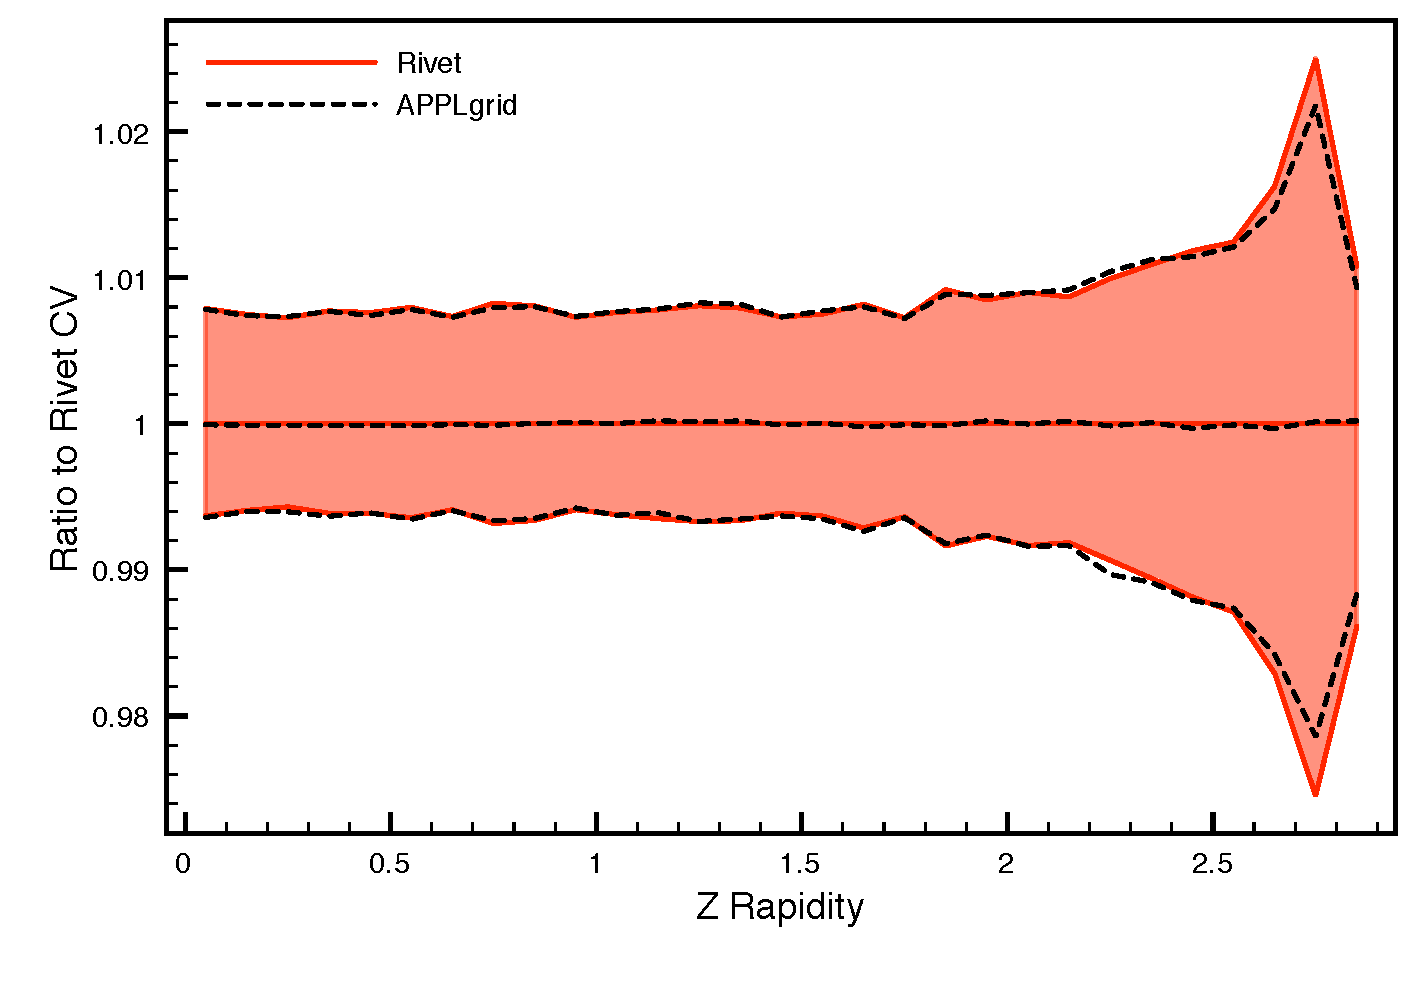
\includegraphics[width=0.45\paperwidth]{100MDYScales_Plot.pdf}
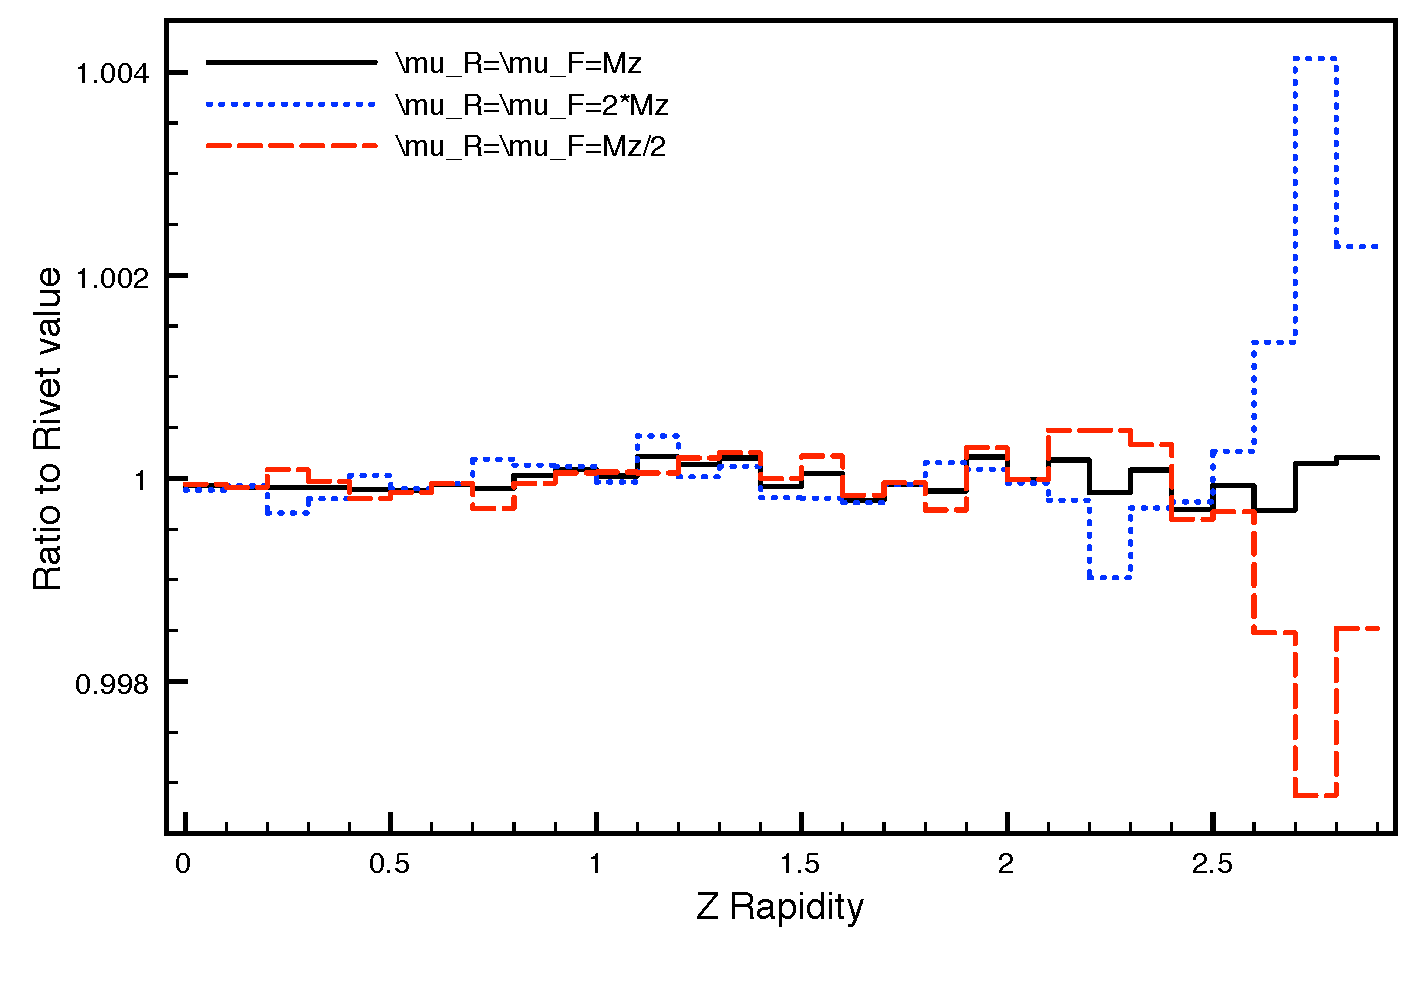
\includegraphics[width=0.45\paperwidth]{100MDYRatioScales_Plot.pdf}\\
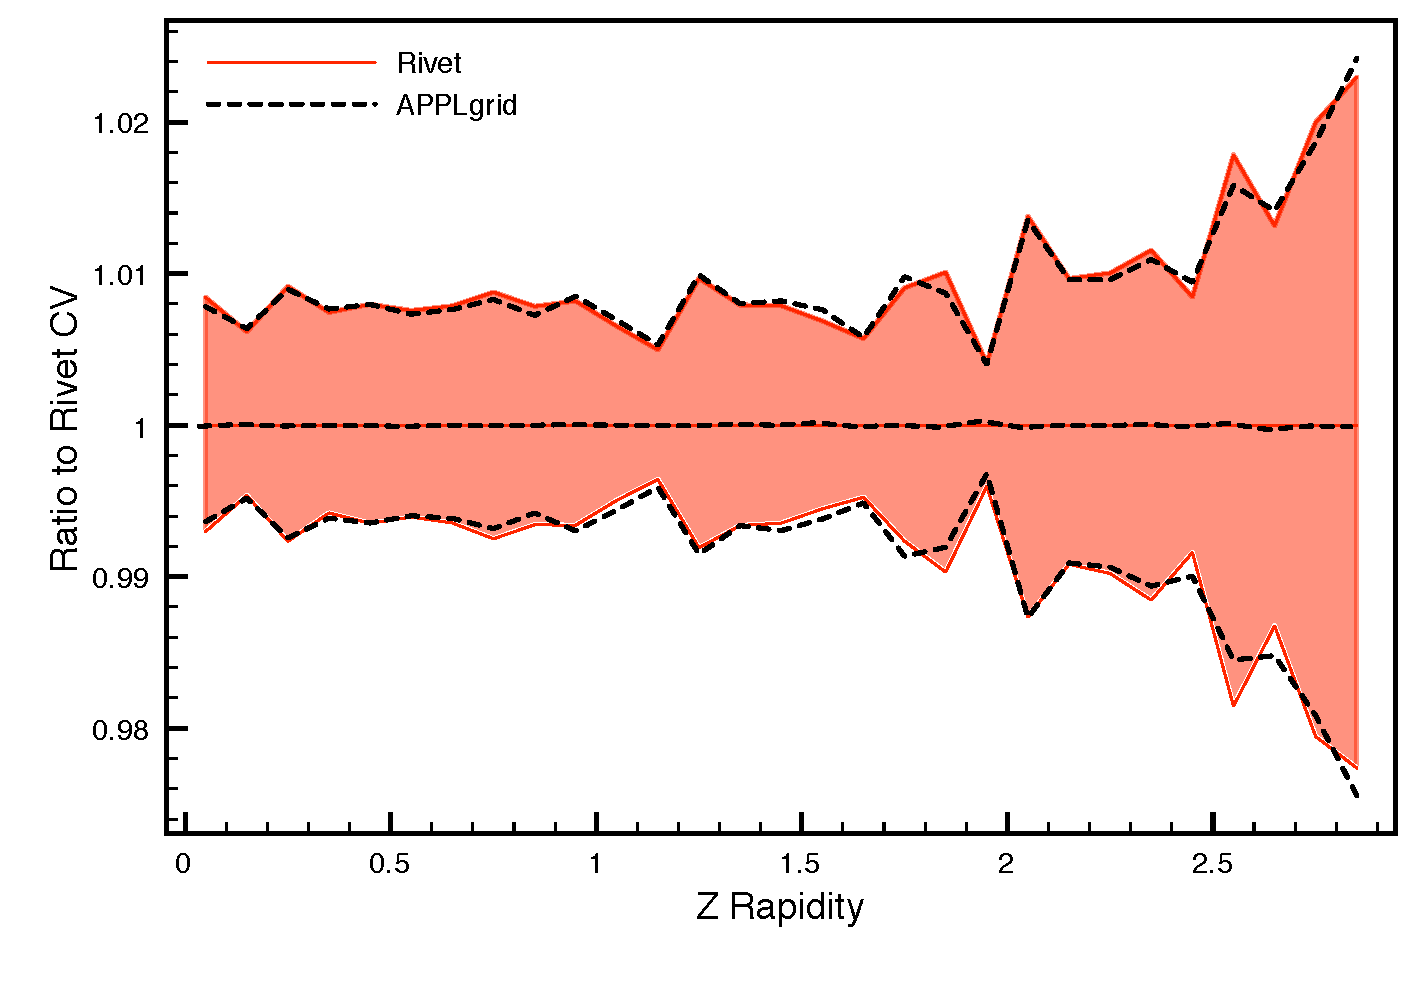
\includegraphics[width=0.45\paperwidth]{10MDYScales_Plot.pdf}
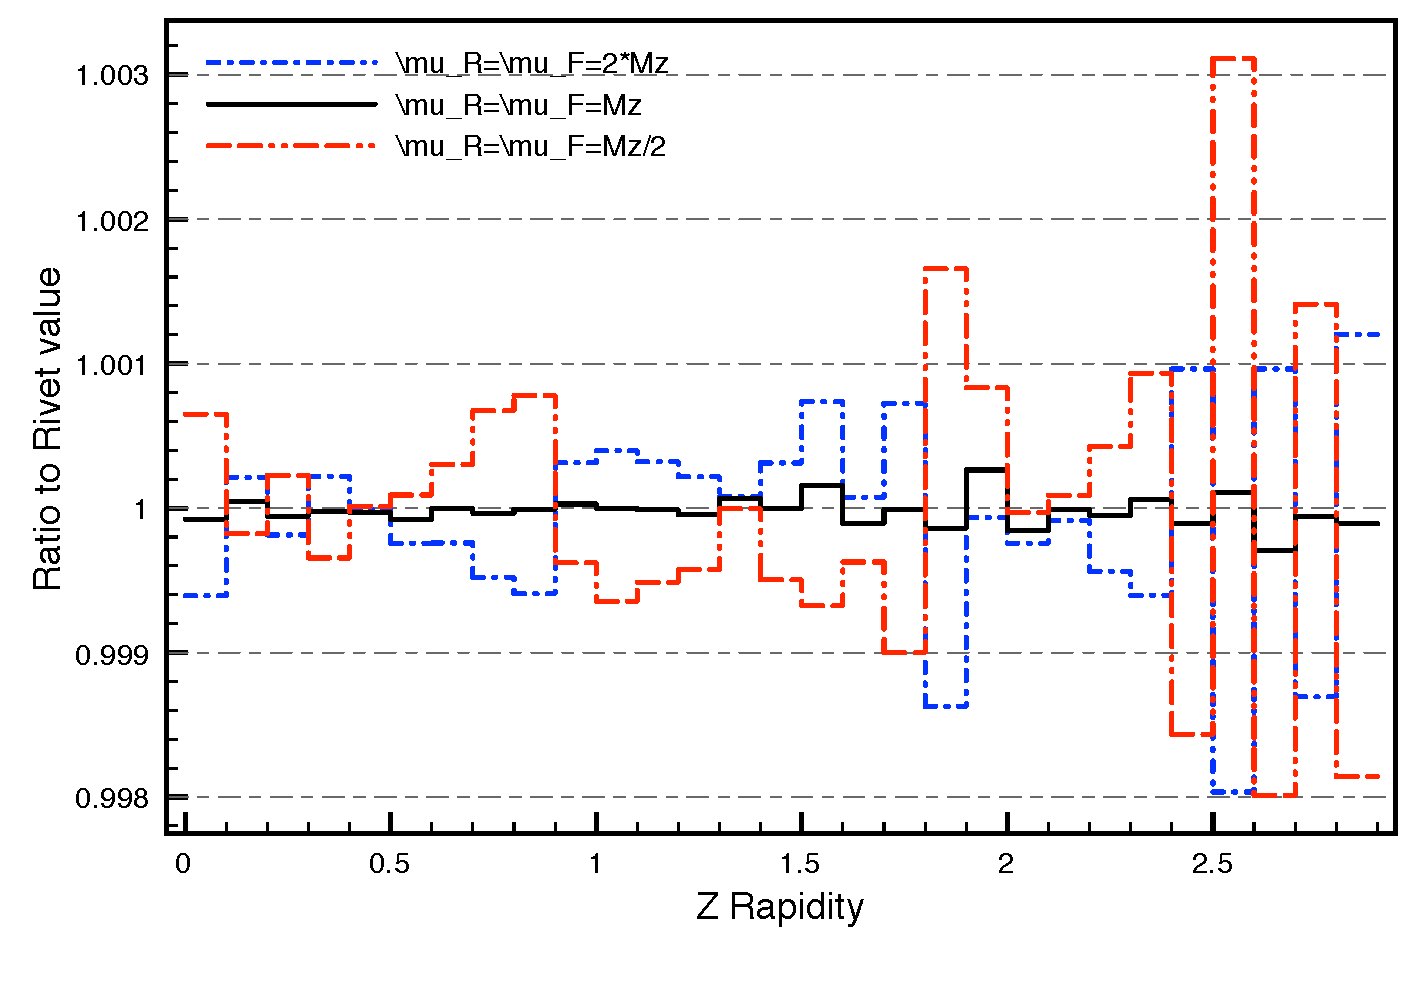
\includegraphics[width=0.45\paperwidth]{10MDYRatioScales_Plot.pdf}
\end{frame}

% End of slides
\end{document} 